\documentclass[9pt,twocolumn,twoside]{../../styles/osajnl}
\usepackage{fancyvrb}
\journal{i524} 

\title{Predicting Customer Churn Using Apache Spark Machine Learning}

\author[1,*]{Yatin Sharma, Diksha Yadav}

\affil[1]{School of Informatics and Computing, Bloomington, IN 47408, U.S.A.}


\affil[*]{Corresponding authors: yatins@indiana.edu, yadavd@iu.edu}

\dates{project-001, \today}

\ociscodes{Prediction, Bigdata, Apache Spark, ML, Hadoop, ,Ansible, Cloudmesh, Analytics}

% replace this with your url in github/gitlab
\doi{\url{https://github.com/cloudmesh/sp17-i524/tree/master/project/S17-IR-P016/report/report.pdf}}


\begin{abstract}
	This report presents a reference implementation to the Customer Churn
	Prediction Project that is built using Apache Spark Machine Learning. In this
	report, we discuss the models used for predicting customer churn along with
	their accuracies. We will also discuss the software deployment on Chameleon and
	Jetstream cloud computing environments using Ansible and Cloudmesh Client
	scripts.
		\newline
\end{abstract}

\setboolean{displaycopyright}{true}

\begin{document}
\setcounter{tocdepth}{5}
\setcounter{secnumdepth}{5}
\maketitle

\tableofcontents % Print the contents section

\section{Introduction}
	One of the most important business metrics is churn rate- describing the rate at which your customers stop doing business with you. Our aim is to build a predictive model which uses data science to predict in advance which customers are at risk of leaving. Such model will allow the company to be proactive and focus on such customers. We used Apache Spark\cite{www-apache-spark} Machine Learning library(ML)\cite{www-Spark-ML} for fitting a predictive model on our dataset. Detailed analysis and modeling was carried out in Python Programming language and different machine learning algorithms were tested on the same dataset. Application deployment was initially done on localhost, followed by deployment on two different clouds. Finally Performance metrics on each of the infrastructure was compared and has been included the report.
	



\section{Architecture}
	Our application was prototyped on smaller dataset locally and was then modified to run on cluster. Fig \ref{Architecture} below describes the runtime architecture of a distributes spark application. 
	
	\begin{figure}[htbp]
		\centering
		\fbox{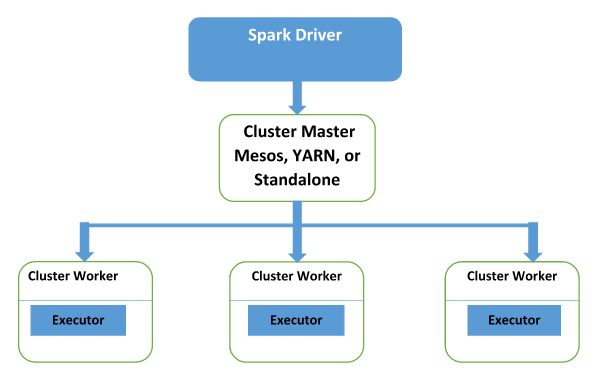
\includegraphics[width=\linewidth]{images/Architecture.png}}
		\caption{Runtime architecture of spark in distributed mode\cite{Learn-Spark}}
		\label{Architecture}
		\end{figure}
			
			

	
	In distributed mode, Spark uses a master/slave architecture with one central coordinator and many distributed workers(2 in our case). The central coordinator is called the driver. The driver communicates with the distributed worker called executors. The driver runs in its own Java Process and each executor is a separate Java process. A driver and its executers are together termed a Spark Application. A Spark application is launched on a set of machines using an external service called cluster manager. We used Hadoop YARN\cite{YARN} as our cluster manager in cloud deployments.
	
\subsection{The Driver}
	The driver is the process where main() method of our program runs. It is the process running the user code that creates a SparkContext, creates RDDs(Resilient Distributed Dataset), and performs transformations and actions.
	
\subsection{Executors}
	Spark executors are worker processes responsible for running individual tasks in a given spark job.Executors have two roles. First, they run the tasks that make up the application and return the result to the driver. Second, they provide in-memory storage for the RDDs.
	
\subsection{Hadoop YARN}
	YARN is cluster manager that provides a data processing framework to run on a shared resource pool, typically on the same node as the Hadoop filesystem( HDFS)\cite{HDFS}. In our project, an HDFS Spark cluster was set up on cloud using Cloudmesh Client.\cite{Cloudmesh} The dataset was stored on the same HDFS system which was then accessed by our spark appication for quick data processing. Using YARN in spark is also straightforward with the help of spark-submit as follows:
	
	\begin{verbatim}
	$ ./bin/spark-submit --master yarn yourapp
	\end{verbatim}	
	
\subsection{Launching a program}
	Spark provides a single script to submit our program to it called spark-submit. Through various options, spark-submit can connect to different cluster managers and control how many resources the application gets. For example following command can be used to launch a spark application.
	\begin{verbatim}
	$ ./bin/spark-submit --class path.to.your.Class 
	--master yarn --deploy-mode cluster [options] 
	<app jar> [app options]
	\end{verbatim}
	
	
	
\section{TECHNOLOGIES}

	Table \ref{table:technologies} lists the set of technologies that were used in building this project.
	
	\begin{table}[h!]
		\centering
		\begin{tabular}[width=\linewidth]{|l l|}
			\hline
			\textit{Technology} & \textit{Usage}  \\  \hline
			\hline 
			\textbf{Python}\cite{www-python} & Development \\
			\hline
			\textbf{Hadoop}\cite{www-hadoop} & Big Data
			Technology  \\
			\textbf{Spark}\cite{www-spark} & Big Data Technology \\
			\hline
			\textbf{Apache Spark ML}\cite{www-Spark-ML} &
			Machine Learning Library \\
			\hline
			\textbf{Cloudmesh Client}\cite{Cloudmesh} &
			Cloud Resource Manager \\
			\hline		
			\textbf{GitHub}\cite{www-github} & Project Repository \\
			\hline
			\textbf{Ansible}\cite{www-ansible} & Application Deployment \\ & $\&$
			Configuration Management \\
			\hline
			\textbf{Chameleon}\cite{www-chameleon},
			\textbf{JetStream}\cite{www-jetstream} & Cloud deployment \\ & $\&$
			Benchmarking \\
			\hline
		\end{tabular}
		\caption{Technologies used}
		\label{table:technologies}
	\end{table}

\begin{itemize}
	\item \textbf{Python}: Python is a high level programming language having
	various popular libraries for data analysis and machine learning algorithms, making it our preferred choice fo the project.
	
	\item \textbf{Hadoop}:  Apache Hadoop is a framework that allows processing and storing huge amounts of data across a distributed resource pool. Therefore, in order to improve overall performance and scalability Hadoop was installed at the foundation of each virtual machine in the cloud.
	
	\item \textbf{Spark}:  Apache Spark is a cluster computing platform designed to be fast and general purpose. It extends the popular MapReduce model to efficiently support more types of computations including interactive queries and stream processing. We will primarily use Spark's machine learning library to build a predictive model on our dataset.
	
	
	\item \textbf{ML}:  ML is Spark’s primary machine learning library. It is DataFrame\cite{DataFrame} based API that makes practical machine learning scalable. The main concepts in Spark ML are:
	
	\begin{enumerate}
		\item {DataFrame} A DataFrame is a Dataset organized into named columns.\cite{DataFrame}
		\item {Transformer} A Transformer is an abstraction that includes feature transformers and learned models. It converts one dataframe into another.\cite{Transformer}
		\item {Estimator} An Estimator is an algorithm which can be fit on a DataFrame to produce a Transformer. For example, training/tuning on a DataFrame and producing a model.
		\item {Pipeline} A Pipeline is specified as a sequence of stages, and each stage is either a Transformer or an Estimator. It represents a workflow, which is run in a specific order.\cite{Pipeline} 
	\end{enumerate}
	
	
	\item \textbf{Cloudmesh Client}: Cloudmesh Client provides an application programming interface(API), which allows us to manage a set of cloud resources. It standardize access to various clouds and clusters. In our project, Cloudmesh Client is used to set up Hadoop virtual cluster with Spark on two cloud environment. Following tasks are performed using Cloudmesh Client:
	
	\begin{enumerate}
		\item {Uploading Public Key-} using Cloudmesh's key add and upload commands.
		\item {Uploading Security Rules-} using Cloudmesh's secgroup commands.  
		\item {Creating Hadooop/Spark Cluster-} using Cloudmesh's deploy command. 
	\end{enumerate}
	
	\item \textbf{GitHub}: GitHub is 'a web-based Git or version control repository and Internet hosting service' \cite{www-github}. We used Github repositories to store our files related to documentation, ansible scripts and python code.
	
	\item \textbf{Ansible}: Ansible is an open source automation platform that automates Application Deployment, and many other IT needs. In our project, Ansible is used to manage the configuration and automate deployment of software stacks on to the clouds. Ansible scripts are run via localhost by providing it with the IP addresses of the cloud VM's set up using Cloudmesh Client.
	
\end{itemize}				


\section{CLOUD INFRASTRUCTURE}
	Two clouds were selected for deployment: Chameleon Cloud and Jetstream. For successful deployment, following applications/utilities were used.
	\subsection{Chameleon Cloud}
		Chameleon  is a collaborative cloud service funded by National Science Foundation primarily meant for research community. In our project three virtual machines were created on this cloud. One acting as master node and the other two as executor nodes for our spark application.
	
	\subsection{Jetstream Cloud}
		Jetstream is a cloud service led by Indiana University’s Pervasive Technology Institute (PTI) in collaboration with other universities \cite{www-jetstream} across the United States. In our project three virtual machines were created on this cloud. One acting as master node and the other two as executor nodes for our spark application.
		
	\subsection{Cloud Hardware Comparison}
		Table 2. below shows a comparison of key computing resources on Chameleon and Jetstream Cloud environment.
	
	\begin{table}[h!]
		\centering
		\begin{tabular}{|c|c c|} 
			\hline
			\textit{Clouds} & \textit{Chameleon} & \textit{Jetstream} \\ 
			\hline
			\hline 
			\textit{CPU} & Intel Xeon & Dual Intel \\ 
			& X5550 & E-2680v3 "Haswell" \\
			\hline 
			\textit{Cores} & 1008 & 7680 \\
			\hline 			
			\textit{RAM} & 5376 GB & 40 Tbr \\ 
			\hline 
			\textit{Speed} & 2.3 GHz & 2.5 GHz\\
			\hline 
			\textit{Storage} & 1.5 PB & 2TB \\
			\hline 

		\end{tabular}
		\caption{Cloud Hardware Specifications.}
		\label{table:clouds}
	\end{table}
	
\section{GETTING STARTED}
	The following section describes the process involved in building the spark application to predict the customer churn.
	
	\subsection{Loading the data}
		The 'Customer Data' used in the project contained 21 columns and 7000 rows. The data was stored in Hadoop distributed file system (HDFS) configured on the cloud cluster. Each row in the dataset represents an observed customer and each column represents attribute of that customer. Dataset was loaded into Spark DataFrame \cite{DataFrame} along with the specified schema. After the dataframe was instantiated, it was queried using SQL queries with the help Pyspark DataFrame API.

	\subsection{Feature Engineering}
		Every single information we use to represent a customer is called a “feature” and the activity of finding useful features is called “feature engineering.” In the Customer data set the data is labeled with two classes – Yes (Churned) and 0
		(Not Churned). The features for each customer consist of:
		\begin{description}
			\item \textbf{Labels-->} Churn: Yes or No
			\item \textbf{Features-->} customerID,gender,SeniorCitizen,Partner,
			Dependents, PhoneService,MultipleLines,InternetService,
			OnlineSecurity,
			OnlineBackup,DeviceProtection,TechSupport,
			StreamingTV,
			StreamingMovies,Contract,PaperlessBilling,
			PaymentMethod,
			MonthlyCharges,TotalCharges		
		\end{description}

	\subsection{Define Feature Array}
		In order for the features to be used by a machine learning algorithm (Spark ML), It is useful for combining raw features and features into a single feature vector, which are vectors of numbers representing the value for each feature. Next, VectorAssembler\cite{VectorAssembler} is used to transform and return a new dataframe with all of the feature columns in a vector column. Finally we use this dataframe to train our model.

	\subsection{Model Training}

	Fig \ref{Workflow} below shows the workflow used in training our machine learning algorithm.

		\begin{figure}[htbp]
		\centering
		\fbox{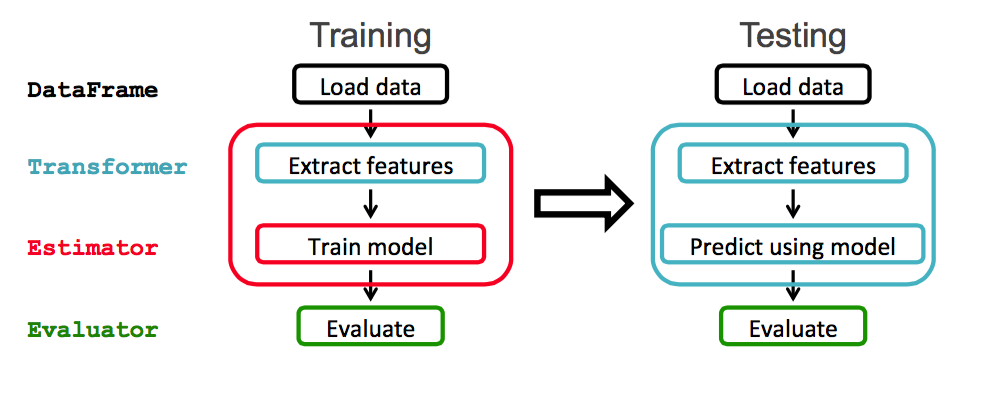
\includegraphics[width=\linewidth]{images/Workflow.png}}
		\caption{Spark ML Workflow \cite{ML-Workflow}}
		\label{Workflow}
		\end{figure}

	We used the following Machine Learning Algorithm and compared them using metrics like accuracy, AUROC and confusion matrix.
		\begin{enumerate}
		\item {Random Forest}
		\item {Decision Tree}  
		\item {Support Vector Machine} 
		\end{enumerate}

	For each of the algorithms, the data was split into training and testing subsets with a ratio of 70 percent for training and 30 percent for testing.The predictive performance of each of the algorithm was evaluated by comparing predictions on the testing data set with true values (known as ground truth) using a variety of metrics such as Accuracy, AUROC and Confusion Matrix.

\section{Model Evaluation}
	We used Spark ML's inbuilt classification evaluators to evaluate the predictions of our algorithms. Table \ref{table:ML} below shows the accuracy for each of the algorithm used.

		\begin{table}[h!]
		\centering
		\begin{tabular}{|c c |} 
		\hline
		\textit{Classification Algorithm} & \textit{Accuracy ($\%$)}\\ 
		\hline
		\hline 
		Decision Tree  &  83.75\\
		\hline  
		Support Vector Machine & 86.82\\
		\hline 
		Random Forest & 84.02\\
		\hline
		\end{tabular}
		\caption{Predictive Accuracy}
		\label{table:ML}
		\end{table}


\section{Deployment}
	The project deployment scripts were designed to be simple and reproducible. The deployment consists of Ansible playbooks and Cloudmesh Client scripts. It is run on user's local machine(Ubuntu 16.04). Deployment scripts will install all the necessary software along with project codes onto the cluster nodes, run spark job on the cloud and finally fetch result on the users local machine. The following section describes how to use the deployment scripts to install and run the project in the cloud.
	
	\subsection{Requirements}
		In order to run the project deployment scripts, one must have Ansible and Cloudmesh Client configured and installed on their local machine. 
	\begin{enumerate}
		\item Cloudmesh Client:		
		In our project Cloudmesh Client is used to set up Hadoop virtual cluster with Spark on two cloud environment. In order to run a virtual machine in the cloud, ~/.cloudmesh/cloudmesh.yaml configuration file should be configured to fill in detail about our cloud accounts such as username, password, project name, etc. Following tasks are performed in our project using Cloudmesh Client:
		
		\begin{enumerate}
			\item {Uploading Public Key-} using Cloudmesh's key add and upload commands.
					\begin{verbatim}
						$ cm key add --ssh
						$ cm key upload
					\end{verbatim}	
					
			\item {Uploading Security Rules-} using Cloudmesh's secgroup commands.  
					\begin{verbatim}
						$ cm secgroup upload
					\end{verbatim}	
			\item {Creating Hadooop/Spark Cluster-} using Cloudmesh's deploy command. 
					\begin{verbatim}
						$ cm cluster define --count 3  
						 --image CC-Ubuntu14.04
						$ cm hadoop define spark
						$ cm hadoop sync
						$ cm hadoop deploy
					\end{verbatim}	
		\end{enumerate}
		
		
		
		
		\item Ansible Scripts:
			In our project, the entire cloud interaction including spark application installation, uploading data, setting up environment, running the spark application, and fetching the result is performed via Ansible playbooks.
			Ansible script was used in the following way:
			
			\begin{enumerate}
				\item \verb|Local Configuration| :
				In the host file the IP address of  remote namenode of the cluster is specified as follows:
					\begin{verbatim}
						[predict]
						129.114.33.144 ansible_ssh_user=cc
					\end{verbatim}

					\item \verb|predict_setup.yaml| :  sets up environment, copies files/code and installs dependencies on the namenode of the cluster. 
					
					
					\item \verb|predict_execute.yaml| :   
					This moves the downloaded data to HDFS through the following command:
					\begin{verbatim}
					$ hdfs dfs  –put <source> <hdfs-folderpath>
					\end{verbatim}
					
					This HDFS file will serve as an input to our spark application. Finally the spark application is submitted to the namenode, which runs it on distributed framework and fetches result from remote to local after job completion.

			\end{enumerate}
			
	\end{enumerate}
		



 \section{Benchmarking}
	After the Hadoop Spark cluster is set up on the cloud, a benchmarking process is run to asses the performance of our deployment and Spark job on the two clouds. Figure \ref{Benchmark2} below compares the time set up environment, install dependencies, run application and fetch result from both the clouds. For measuring the time we used shell script to calculate the time elapsed between begin and completion of Ansible playbooks.
		\begin{figure}[htbp]
			\centering
			\fbox{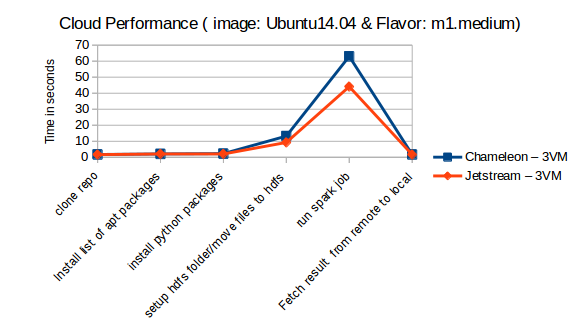
\includegraphics[width=\linewidth]{images/Benchmark2.png}}
			\caption{Time Comparison in seconds}
			\label{Benchmark2}
		\end{figure}
	
	First time installation for the dependencies and apt-packages takes considerable amount of time(10-15 minutes) and hence are not included in the above comparison graphs. Specifically, Spark application performs 23 percent faster on 3 node Jetstream cluster when compared to similar cluster on chameleon.
\section{Conclusion}
	We have built and tested a fully automated program to configure, deploy and run Apache Spark's Machine Learning algorithm for customer churn prediction on two cloud environments(Chameleon and Jetstream). The use of Ansible Galaxy to automate deployment and Cloudmesh Client to setup Virtual Cluster on cloud helped in reproducibility and scalability.


\section{ACKNOWLEDGMENT}
	The authors would like to thank Gregor von Laszewski and course TA's for their technical support and guidance.
	
\section{WORK BREAKDOWN}
	The work in this project was equally distributed between the following authors.
	
	\textbf{Diksha Yadav}: Data analysis and building   Spark pipeline for machine learning algorithm in stand alone mode, benchmarking and troubleshooting.
	
	\textbf{Yatin Sharma}: Code deployment, building ansible scripts, benchmarking and troubleshooting.

\bibliography{references}
\end{document}
